\documentclass[compress, smaller, serif, 9pt]{beamer}


\mode<presentation>
{
  \usetheme{Montpellier}
  %\setbeamercovered{transparent}
  % or whatever (possibly just delete it)
}
% or whatever
%\setbeamertemplate{footline}[frame number]
\beamertemplatenavigationsymbolsempty
\beamertemplatetransparentcovereddynamic

\usepackage[english,frenchb]{babel}
\usepackage[utf8]{inputenc}
% or whatever
%\setbeamertemplate{footline}[frame number]
\beamertemplatenavigationsymbolsempty
\beamertemplatetransparentcovereddynamic
\usefoottemplate{%
       \tinycolouredline{blue!03}%
       {
           \hspace{11.5cm}{\color{black!50} {\insertframenumber $/$ \inserttotalframenumber} \hfill}
       }%
}


% Definitions
%\input{def}
% Raccourcis
%\input{raccourci}

% Beamer settings
%\setbeamercolor{structure}{fg=myem!120}
%\setbeamercolor{example}{bg=LightYell,fg=StroYell}

% \setbeamercolor{alerted text}{fg=lightred}
% \setbeamertemplate{blocks}[rounded][shadow=true]
% \newcommand{\exampletext}[1]{{\usebeamercolor[fg]{example text} #1}}
% \newcommand{\structuretext}[1]{{\usebeamercolor[fg]{structure} #1}}
% \usefonttheme[onlymath]{serif}
% \renewcommand{\thefootnote}{\fnsymbol{footnote}}

%\setbeamerfont{sidebar}{5pt}

\usepackage{amssymb}
%\usepackage[T1]{fontenc}
\usepackage{amsmath,amsthm,bm}
\usepackage{pgf}


\graphicspath{{./Figs/S06/}{./Figs/S05/},{./Figs/S04/},{./Figs/S03/}}

\usepackage[normal]{subfigure}
\newcommand{\goodgap}{%
    \hspace{\subfigtopskip}%
    \hspace{\subfigbottomskip}}

% les macros
\newcommand{\exampletext}[1]{{\usebeamercolor[fg]{example text} #1}}
\newcommand{\structuretext}[1]{{\usebeamercolor[fg]{structure} #1}}

\newcommand{\bydef}{\stackrel{{def}}{=}}
\newcommand{\ici}{\tcb{$\blacktriangleright \;$}}
\newcommand{\icir}{\alert{$\blacktriangleright \;$}}
\newcommand{\iciex}{\exampletext{$\blacktriangleright \;$}}
\usepackage{pifont}
\newcommand{\doigt}{\structuretext{\noindent \Pisymbol{pzd}{43}}}
\newcommand{\doigtr}{\alert{\noindent \Pisymbol{pzd}{43}}}
\newcommand{\doigtex}{{\exampletext{\noindent \Pisymbol{pzd}{43}}}}


\setbeamerfont{block title}{size={\normalsize}}

\newcommand{\bx}{{\boldsymbol{x}}}
\newcommand{\bX}{{X}}
\newcommand{\bd}{{\boldsymbol{d}}}
\newcommand{\bD}{{D}}
\newcommand{\ba}{{\boldsymbol{a}}}
\newcommand{\bAl}{A}
\newcommand{\bA}{{A}}
\newcommand{\bu}{{\boldsymbol{u}}}
\newcommand{\bU}{{{U}}}
\newcommand{\bv}{{\boldsymbol{v}}}
\newcommand{\bV}{{{V}}}
\newcommand{\bSig}{{{\Sigma}}}
\newcommand{\bE}{{{E}}}
\newcommand{\bI}{{{I}}}
\newcommand{\br}{{\boldsymbol{r}}}





\title[Statistical Learning]{Machine/Statistical Learning}

\subtitle{Lecture 6: Dictionnary Learning}


%\author[Florent Chatelain]{Florent Chatelain}
\institute{Filière SICOM, 3A}
%\logo{\includegraphics[width=.2\textwidth]{logoE3}}

\date{}


%

\begin{document}

\maketitle

\section{Dictionary problem}

\begin{frame}
  \frametitle{Reminder of regression and sparsity}
  
  \begin{itemize}
   \item $\bx \in \mathbb{R}^p$ $\leftarrow$ observations, 
   \item $\bD \in \mathbb{R}^{p \times K}$ $\leftarrow$ design/regression matrix,
  \end{itemize}
  
  


  \begin{block}{Regression problem}
  Find coefficient vector $\ba\in\mathbb{R}^K$ s.t. \quad $\bx \approx \bD \ba$, \quad i.e. $\| \bx - \bD \ba \| \le \epsilon$
  \begin{itemize}
     \item[\doigt] regularization/model selection: \structuretext{sparsity} constraint
     $$ \min_{\ba} \| \bx-\bD\ba\|_2^2 \quad \textrm{s.t. } \textrm{Pen}(\ba) \le T, \quad \textrm{with e.g.}$$
     \item $\textrm{Pen}(\ba) = \| \ba\|_1$ $\leftarrow$ \structuretext{$\ell_1$} norm,
     \item $\textrm{Pen}(\ba) = \| \ba\|_0 \equiv \#\{ i \ : \ 1\le i \le K \textrm{ and } \structuretext{\ba_i \ne 0} \}$ $\leftarrow$ \structuretext{$\ell_0$} {\em pseudo-norm}, i.e. number of non-zero components for $\ba$
  \end{itemize}
    \end{block}
    
\end{frame}



\begin{frame}
  \frametitle{Dictionary problem}

  \begin{block}{Assumptions}
  \begin{itemize}
     \item Inputs: $\bx_i \in \mathbb{R}^p$, for $i=1,\ldots,n$, \quad $\leftarrow$ learning set
  \end{itemize}
  \end{block}
    \begin{block}{Objective}
  ``Inverse'' the regression problem, i.e. \structuretext{find $\bD \in \mathbb{R}^{p\times K}$} ensuring a \structuretext{sparse} approximation/representation of
  the learning set $\bx_1,\ldots,\bx_n$
  $$ \bx_i \approx \bD \ba_i, \ \textrm{ for } i=1,\ldots,n,  \quad \textrm{s.t.}$$
  \vspace{-5mm}
  \begin{itemize}
     \item \alert{$K \ll n$} $\leftarrow$ sparsity of the representation 'basis' ($\sim$ low rank constraint)
     \item \alert{$\|\ba_i\|_0 \le T$}, for $i=1,\ldots,n$ $\leftarrow$ sparsity of the coefficients
   \end{itemize}     
    \end{block}
\begin{block}{Dictionary terminology}
 \begin{itemize}
     \item $\structuretext{\bD} \equiv \begin{pmatrix}\bd_1 |& \ldots&| \bd_K\\  \end{pmatrix} \in \mathbb{R}^{p\times K}$ $\leftarrow$ \structuretext{dictionary}
     s.t.  {$K \ll n$ (low rank)}
     \item $\structuretext{\bd_k} \in  \mathbb{R}^{p}$ $\leftarrow$ \structuretext{atoms} with $k=1,\ldots,K$ (column vectors of $\bD$)
     \item $\structuretext{\ba_i} \in  \mathbb{R}^{K}$ $\leftarrow$ \structuretext{coefficients} of $\bx_i$ s.t. {$||\ba_i||_0 \le T$ (sparsity)} 
  \end{itemize}
        \end{block}


    
\end{frame}




\begin{frame}
  \frametitle{Dictionary vs Orthornormal Basis (ONB)}

  \begin{block}{Orthornormal Bases (ONB)}
  Lots of good properties for ONB (e.g. Fourier, orthonormal wavelets,\ldots):
  \begin{itemize}
     \item uniqueness of the decomposition ($n$ coefficients to represent a $n$-dimensional  vector),
     \item existence of fast transforms,
     \item projections to obtain approximate representations, \ldots
  \end{itemize}
  \alert{But} not necessarily good for sparse representations
  \begin{itemize}
    \item[\doigtr] e.g. sums of sinusoids + spikes  (+ steps) are  not sparse in either Fourier or identity bases...
    \end{itemize}
  \end{block}
    
    \begin{block}{Dictionary}
    Change of mindset
    \begin{itemize}
     \item loose uniqueness of representation using \structuretext{overcomplete/redundant} bases 
  \item[\doigt] get \structuretext{sparser} representations in return!
      \end{itemize}
    \end{block}
    
\end{frame}


\begin{frame}
  \frametitle{Recap: Dictionary and Sparse representations}

  \begin{block}{Hypotheses}
  \begin{itemize}
     \item Inputs: $\bx_i \in \mathbb{R}^p$, $1 \le i \le n$,  
     \quad $\rightarrow$ $\bX=\begin{pmatrix} \bx_1 | &\hspace{-2mm }  \ldots \hspace{-2mm }  & |\bx_n\\  \end{pmatrix} \in \mathbb{R}^{p \times n}$
  \end{itemize}
  \end{block}
  \vspace{-2mm}
    \begin{block}{Objective: sparse representation/factorization  $X \approx \bD \bAl$}
   \vspace{-2mm}
  \begin{center}
     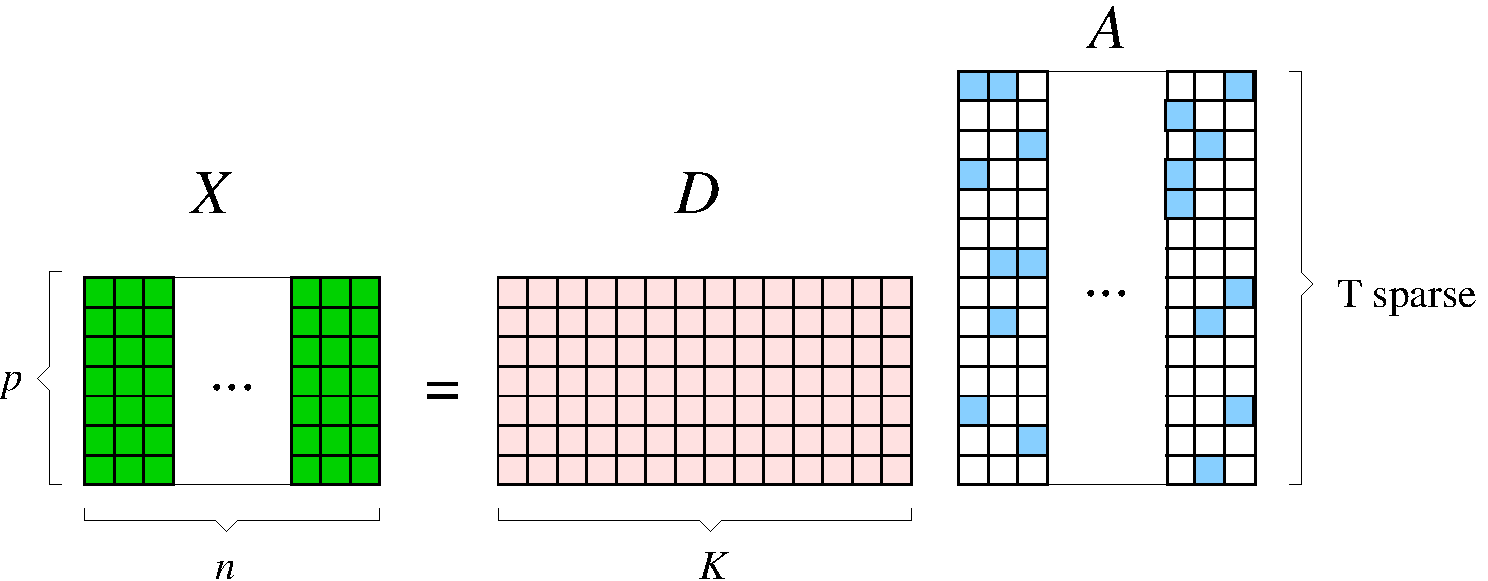
\includegraphics[width=.7\textwidth]{dict_learn_pb2.pdf}%\\
     %\textcolor{blue}
     \vspace{-2mm}
  \end{center}%\hspace*{-5mm}
  %\vspace{-2mm}
  {
  \setlength{\parindent}{-5em} 
  \begin{itemize}
     \item \hspace{-2mm } $\structuretext{\bD} \equiv \begin{pmatrix}\bd_1|&\hspace{-3mm }  \ldots \hspace{-3mm } &| \bd_K\\  \end{pmatrix} \in \mathbb{R}^{p\times K}$ $\leftarrow$ \structuretext{dictionary} (redundant), with
     \alert{$K \ll n$}.
     \item \hspace{-2mm } $\structuretext{\bd_k} \in  \mathbb{R}^{p}$ $\leftarrow$ \structuretext{atoms} with $k=1,\ldots,K$
     \item \hspace{-2mm } $\structuretext{\bAl} \equiv \begin{pmatrix}\ba_1|&\hspace{-3mm } \ldots \hspace{-3mm }  &| \ba_n\\  \end{pmatrix} \in \mathbb{R}^{K \times n}$ $\leftarrow$ \structuretext{coefficients} s.t. 
     $\bx_i \approx \bD \ba_i$ with  \alert{$||\ba_i||_0 \le T$ } 
     \item[\doigt] only the observations $\bx_i$ are known: \structuretext{unsupervised} problem
  \end{itemize}
  }
    \end{block}
    
\end{frame}


\begin{frame}
  \frametitle{Formalizing the dictionary learning problem}
  
  \begin{block}{Cost criterion with sparsity constraints}
  \vspace{-4mm}
  \begin{align*}
     \min_{\structuretext{\bD},\structuretext{\{\ba_i\}}} J\left(\bD,\{\ba_i\}\right) & 
     \equiv \sum_{i=1}^n \| \bx_i - \bD \ba_i \|_2^2  = \structuretext{ \| \bX-\bD \bAl\|^2_F},\\
     \textrm{s.t. }  \structuretext{ \textrm{Pen}(\ba_i) \le T }&  \quad \textrm{for } i=1,\ldots,n
  \end{align*}
  \vspace{-4mm}
  \begin{itemize}
  \item $\bX = \begin{pmatrix}\bx_1|&\hspace{-2mm }  \ldots \hspace{-2mm } &| \bx_n\\  \end{pmatrix} \in \mathbb{R}^{p\times n}$, 
  \quad $\bD = \begin{pmatrix}\bd_1|&\hspace{-2mm }  \ldots \hspace{-2mm } &| \bd_K\\  \end{pmatrix} \in \mathbb{R}^{p\times K}$, \quad 
   $\bAl = \begin{pmatrix}\ba_1|&\hspace{-2mm }  \ldots \hspace{-2mm } &| \ba_n\\  \end{pmatrix} \in \mathbb{R}^{K \times n}$,\\
   \item $\|M\|_F^2 \equiv \sum_{i,j} m_{ij}^2$ $\leftarrow$ Frobenius norm   
  \end{itemize}
\end{block}


  \begin{block}{Identifiability issue}
  \begin{itemize}
     \item[Pb:] atoms $\bd_k$ and their associate coefficients $\ba^k \in \mathbb{R}^{1\times n}$ ($k$th line of $\ba$) are defined up to a scaling factor in the factorization criterion
     \item[\doigtr] atoms are assumed to be \alert{normalized}, i.e. \alert{$\|\bd_k\|_2 =1$}, for $k=1,\ldots,K$      
  \end{itemize}
  \end{block}
    
\end{frame}


\begin{frame}
  \frametitle{Optimizing the factorization criterion}
  \begin{block}{Alternate minimization method}
    \vspace{-4mm}
  \begin{align*}
     \min_{\structuretext{\bD},\structuretext{\{\ba_i\}}} J\left(\bD,\{\ba_i\}\right)= \structuretext{ \| \bX-\bD \bAl \|^2_F}, \quad
     \textrm{s.t. }  \structuretext{ \textrm{Pen}(\ba_i) \le T }
  \end{align*}
  \vspace{-2mm}
  
  Joint minimization w.r.t. $\bAl$ and $\bD$ split into $2$ simpler separated steps 
  \begin{enumerate}
   \item \structuretext{sparse coding} to estimate the coefficients $\bAl$  for a given dictionary $\bD$,
   \item \structuretext{dictionary $\bD$ update} performed atom-by-atom, for a given $\bAl$
   \item[\doigt] repeat 1) and 2) until a stopping criterion
  \end{enumerate}
  \end{block}
  
  
 \begin{block}{Optimization issues}
\begin{itemize}
 \item when $\textrm{Pen}(\ba_i)= \| \ba_i \|_0$ $\leftarrow$ \alert{NP-hard} combinatorics problem...
 \item joint minimization w.r.t. $\bD$ and $\{\ba_i\}_{1\le i\le n}$ $\leftarrow$ \alert{non-convex} problem
 \item[\doigtr] \alert{sub-optimal} solution around an initial value for $\bD$ (cf clustering)  
\end{itemize}

\end{block}
    
\end{frame}

\section{Sparse coding}


\begin{frame}
  \frametitle{Sparse coding: update of the coefficients $\ba$}
  
  \begin{description}[align=left]
   \item[Assumption:] $\bD$ fixed
   \item[Objective:] find sparse $\bAl^{\star}$ minimizing $J(\bAl) \equiv J(\bD,\bAl)= \| \bX-\bD\bAl\|^2_F$ %with sparsity constraints
   %\item[\doigt] linear regression problem  with sparsity constraints
  \end{description}
  \begin{itemize}
  \item[\doigt] linear regression problem \structuretext{on each $\ba_i$} with \structuretext{sparsity constraints}
\end{itemize}

  \begin{block}{Basis Pursuit (BP)}
    Convex \structuretext{relaxation} of the $\ell_0$ pseudo-norm with the $\ell_1$ norm:
    $$
    \bAl^{\star} = \min_{\bAl} \| \bX-\bD\bAl\|^2_F + \lambda \sum_{i=1}^n \| \ba_i \|, \quad \textrm{ where } \lambda >0, 
    $$
    \vspace{-4mm}
 \begin{itemize}
   \item convex problem on $\bAl$, with Lasso solutions for $\ba_i$, $i=1,\ldots,n$
   \item[\doigt] Online Dictionary Learning (ODL) algorithm (Mairal {\em et al.}, 2009) 
  \end{itemize}
  \end{block}
  
   \begin{block}{(Orthogonal) Matching Pursuit (OMP)}
    Sparse \structuretext{approximate}  (sub-optimal) solution of the $\ell_0$ minimization problem  using a greedy algorithm to select the ``best matching'' atoms
  \end{block}
 
    
\end{frame}


\begin{frame}
  \frametitle{Orthogonal Matching Pursuit}
  Let $\bD_{\Gamma}$ be the sub dictionary composed of the only atoms $\bd_{k}$ s.t. $k \in \Gamma$ 
  \begin{enumerate}
   \item \textbf{Initialization:} $\Gamma= \emptyset$, $\br= \bx_i$ (sweep on the observations $\bx_i$)

   \item \textbf{for } $iter=1,\ldots,T$ \textbf{do}
   \item \quad Select the best matching atom, i.e. most correlated with the residuals 
   $$ \widehat{k} \leftarrow \max_{1\le k \le K} | \br^T \bd_k |$$
   \item \quad Update the active  set: \quad
    $\Gamma \leftarrow \Gamma \cup \{ \widehat{k} \}$
   \item \quad Update the residuals: \quad
   $\begin{displaystyle} \br \leftarrow \left( \bI_p - \bD_{\Gamma} ( \bD_{\Gamma}^T \bD_{\Gamma} )^{-1} \bD_{\Gamma}^T \right) \bx_i,
    \end{displaystyle}$ 
   %\item \qquad Update the coefficients
   %$$ \ba \leftarrow ( \bD_{\Gamma}^T \bD_{\Gamma} )^{-1} \bD_{\Gamma}^T  \bX,$$ 
   \item \textbf{endfor}
   \item \textbf{Output:} $\ba_i \equiv$ coefficients of the orthogonal projection of $\bx_i$ on the 
   space spanned by $\bD_{\Gamma}$
  \end{enumerate}
\medskip

  \begin{itemize}
  %\item $\bD_{\Gamma}$ is the sub dictionary composed of the only atoms $d_{k}$ s.t. $k \in \Gamma$ 
  \item[\doigt] residuals \structuretext{orthogonal} to the sparse signal approximation $\bD_{\Gamma}\ba_i$
  \item[\doigt] by construction, $\textrm{card}\,(\Gamma)=T$ $\Rightarrow$ \structuretext{$\|\ba_i\|_0 \le T$}
 \end{itemize}

\end{frame}


\section{K-SVD algorithm}

\begin{frame}
  \frametitle{K-SVD algorithm outline}
  
  \begin{enumerate}
   \item preliminary tools: SVD and low rank approximation
   %\item revisiting the K-means algorithm
   \item K-SVD dictionary update and  K-SVD algorithm
  \end{enumerate}

 \end{frame} 

\begin{frame}
  \frametitle{Singular Value Decomposition (SVD)} 
  
  Let $\bX \in \mathbb{R}^{n \times m}$ be a real rectangular matrix. There exists a factorization, called a singular value decomposition of $\bX$, of the form
  $$ \bX= \bU \bSig \bV^T, \quad \textrm{ where}$$
  \vspace{-3mm}
  \begin{itemize}
   \item $\bU \in  \mathbb{R}^{n \times n}$ is \structuretext{orthonormal} ($\bU\bU^T= \bU^T\bU= \bI_n$) $\leftarrow$ matrix of left-singular vectors $\bu_k\in \mathbb{R}^n$ s.t. 
   $\bU=(\bu_1|\ldots|\bu_n)$, \vspace{1mm}
   \item $\bV \in  \mathbb{R}^{m \times m}$ is \structuretext{orthonormal} ($\bV\bV^T= \bV^T\bV= I_m$) $\leftarrow$ matrix of right-singular vectors $\bv_k \in \mathbb{R}^m$ s.t. 
   $\bV=(\bv_1|\ldots|\bv_m)$, \vspace{1mm}
   \item $ \bSig \in  \mathbb{R}^{n \times m}$ is a rectangular \structuretext{diagonal} matrix with non negative diagonal entries $ \structuretext{\Sigma_{ii} \equiv \lambda_i \ge 0}$
   for $i=1,\ldots,\min(n,m)$\vspace{1mm}
   \item[\doigt] the $\lambda_i$'s are \structuretext{uniquely defined} and called the \structuretext{singular values} of $\bX$
   \item[\doigt] By convention, these singular values are sorted in descending order: $$\lambda_1 \ge \ldots \ge \lambda_{\min(n,m)} \ge 0$$
  \end{itemize}

  
\end{frame}

\begin{frame}
  \frametitle{Singular value decomposition (SVD) and principal components analysis (PCA)} 
  
   $\bX\in \mathbb{R}^{n \times m}$ with SVD $\bX=\bU \bSig \bV^T$
  \begin{block}{Eigendecomposition of Gram matrices}
   %Let $X=\bU \bSig \bV^T$ be the SVD of $X \in \mathbb{R}^{n \times m}$,  where $ \lambda_1 \ge \ldots \ge \lambda_{\min(n,m)} \ge 0$ are the singular values (diagonal entries of $\bSig$). Then 
   Gram matrices express as
   $$\begin{array}{lll}
    \bX^T\bX &= \bV \bSig^T \bU^T \bU \bSig \bV^T&= \bV \left(\bSig^T \bSig\right) \bV^T,\\
    \bX\bX^T &= \bU \bSig \bV^T \bV \bSig^T \bU^T  &= \bU \left(\bSig \bSig^T\right) \bU^T,\\
   \end{array}$$
   where $\bSig^T \bSig \in \mathbb{R}^{m \times m}$ and $\bSig \bSig^T \in \mathbb{R}^{n \times n}$ are square diagonal
   \begin{itemize}
        %\item columns of $\bV$ (right-singular vectors) are \structuretext{eigenvectors} of $\bX^T\bX=\bV \left(\bSig^T \bSig\right) \bV^T$,
        \item right-singular vectors of $\bX$ are \structuretext{eigenvectors} of $\bX^T\bX=\bV \left(\bSig^T \bSig\right) \bV^T$,
        \item left-singular vectors of $\bX$ are \structuretext{eigenvectors} of $\bX\bX^T=\bU \left(\bSig \bSig^T\right) \bU^T$,
        \item non-zero singular values $\lambda_i$'s are the \structuretext{square roots of the non-zero eigenvalues} of $\bX^T\bX$ or $\bX\bX^T$
        \item[\doigt] SVD yields \structuretext{principal components analysis} (PCA) decomposition
  \end{itemize}
  \end{block}
  
   
  
\end{frame}



\begin{frame}
  \frametitle{Singular Value Decomposition (SVD) and low rank approximation} 
  
   \begin{itemize}
    \item $\bX\in \mathbb{R}^{n \times m}$ with SVD $\bX=\bU \bSig \bV^T$
    \item[\doigt] left-singular vectors $\bu_k\in \mathbb{R}^n$ of $\bX$ are the columns of $\bU$, for $k=1,\ldots,n$
    \item[\doigt] right-singular vectors  $\bv_k\in \mathbb{R}^m$ of $\bX$ are the columns of $\bV$, for $k=1,\ldots,m$
   \end{itemize}
 
   

    \begin{block}{Eckart–Young–Mirsky theorem}
    For the Frobenius norm ($\|M\|^2_F= \sum_{i,j} m_{i,j}^2$), the solution to the \structuretext{low-rank approximation} problem \quad  
    $\begin{displaystyle} \min_{\hat{\bX}} \| \bX- \hat{\bX} \|_F^2 \quad \textrm{s.t.} \ \operatorname{rank}( \hat{\bX} ) \le r,\end{displaystyle}$
   is \vspace{-3mm}
    $$% \begin{displaystyle}
      \structuretext{\hat{\bX} = \sum_{k=1}^r \lambda_k \bu_k \bv_k^T}, 
    %\end{displaystyle}
    \vspace{-2mm}
    $$
    where $\lambda_k$, $\bu_k$ and  $\bv_k$ are the first \structuretext{singular values and left/right-singular vectors} of $\bX$, for $k=1,\ldots,r\le \min(m,n)$. 
    
    
  \end{block}
  
\end{frame}


\begin{frame}
  \frametitle{Dictionary update: K-SVD algorithm (Aharon {\em et al.}, 2006)}
  
  \hspace*{-2mm} \structuretext{Objective:} For a given $\bAl$, find  $\bD$ minimizing $J(\bD) \equiv J(\bD,\bAl)= \| \bX-\bD\bAl\|^2_F$\\
  
  \medskip
  Sweep on the atoms $\bd_k$ that are sequentially updated, for $k=1,\ldots K$, as $$\min_{\bd_k} \| \bX-\bD\bAl\|^2_F= \| \bE^k - \bd_k \ba^k \|_F^2$$
  %Fixing all the columns of $\bD$ except the $k$th one, it comes that 
  %$\bX-\bD\ba= E_k - \bd_k \ba^k$ 
  %where
  \vspace{-3mm}
  \begin{itemize}
   \item $\ba^k\in \mathbb{R}^{1 \times n}$ is the $k$th \structuretext{line} of $\bAl$, 
   \item $\bE^k=\bX- \sum_{l\ne k} \bd_l \ba^l \in \mathbb{R}^{p \times n} $, 
   \item $\bd_k \ba^k \in \mathbb{R}^{p \times n}$ is a \structuretext{rank $1$ matrix}
  \end{itemize}
  
  
  
  
  \begin{block}{Atoms (and coefficients) update}
  Best rank $1$ approximation of $\bE^k$ obtained from its  \structuretext{SVD}  as $ \lambda_1 \bu_1 \bv_1^T$, 
  \begin{itemize}
   \item $\lambda_1 \equiv$ largest singular value, $\bu_1$ and $\bv_1^T$ $\equiv$ associated singular vectors
  
  \item[\doigt] $\bd_k=\bu_1$ $\leftarrow$ unit norm vector by construction
  \item[\doigt] $\ba^k= \lambda_1 \bv_1^T$ \alert{$\leftarrow$ Pb:} there is no reason for the updated  $\ba^k$ to be \alert{sparse!}
  \end{itemize}
  \end{block}

\end{frame}


\begin{frame}
  \frametitle{Dictionary update: K-SVD algorithm (Aharon {\em et al.}, 2006)}
  
  
  \begin{block}{K-SVD solution to enforce sparsity of the coefficients}
  For updating the $k$th atom restrict attention to the only observations $\bx_i$ for which the atom is active, i.e. data and dictionary  columns with indexes in
  \vspace{-1mm}
  $${\Gamma}_k=\{i\ : \: \alpha^k_i \ne 0 \}$$
  \vspace{-4mm}
  \begin{itemize}
   \item $\ba^k_{\Gamma_k}\in \mathbb{R}^{|\Gamma_k|} $ is the vector of the only non zero components of $\ba^k\in \mathbb{R}^{n} $
   \item $\bE^k_{\Gamma_k} \in \mathbb{R}^{n \times |\Gamma_k|}$ is the matrix obtained by retaining the only 
   column vectors of $\bE^k= \bX- \sum_{l\ne k} \bd_l \ba^l$ with column index $i \in \Gamma_k$
   \item $\lambda_1 \equiv$ largest singular value, $\bu_1$ and $\bv_1^T$ $\equiv$ associated singular vectors of the SVD
   of \structuretext{$\bE^k_{\Gamma_k}$}
  \end{itemize}
  \end{block}
  
  \begin{block}{K-SVD atoms (and coefficients) update}
  \begin{itemize}
  \item $\bd_k \leftarrow \bu_1$  (unit norm vector by construction)
  \item $\ba^k_{\Gamma_k} \leftarrow$ $\lambda_1 {\bv_1}^T$  (hence $\ba^k$ remains as \structuretext{sparse}  as sparse coding outputs)  
  \item[\doigt] both atoms and coefficients are updated during the K-SVD dictionary update step
  \end{itemize}
  \end{block}


\end{frame}



\begin{frame}
  \frametitle{K-SVD algorithm}
  
  \begin{enumerate}
  \setcounter{enumi}{-1}
   \item \structuretext{Initialize} dictionary $\bD^{(0)}$ using union of ONBs elements / randomly by picking $K$ observations
   \item \structuretext{Sparse coding:} computation of the coefficients $\ba_i$ for each $\bx_i$ given $\bD^{(t-1)}$
   (usually using OMP with $\|\ba_i\|_0 \le T$)
   \item \structuretext{Dictionary update:} for each atom $\bd_k \in \bD^{(t-1)}$, $1\le k \le K$ 
   \begin{itemize}
    \item Define the set of active entries $\Gamma_k=\{i\ : \ \alpha_i^k \ne 0 \}$
    \item Compute $\bE^k= \bX- \sum_{l\ne k} \bd_l \ba^l$ and its restriction $\bE^k_{\Gamma_k}$ to columns in $\Gamma_k$
    \item Compute the first largest singular value $\lambda_1>0$ of $\bE^k_{\Gamma_k}$, and the associate left and right singular vectors $\bu_1$ and $\bv_1$
    \item Update the $k$-th atom and the associated coefficients 
    $\begin{array}{lll} \bd_k &\leftarrow &\bu_1,\\
    \ba^k_{\Gamma_k} &\leftarrow &\lambda_1 \bv_1^T
    \end{array}$
   \end{itemize}
  \end{enumerate}
  \begin{itemize}
    \item Repeat steps $1$ and $2$ for $t=1,\ldots$ until convergence
\end{itemize}
\end{frame}



\begin{frame}
  \frametitle{Properties of K-SVD algorithm}
  
  
  \begin{block}{Convergence}
   Convergence to a \structuretext{local minimum} guaranteed if the sparse coding step always decrease the empirical quadratic error
   $\|\bX-\bD\bAl\|^2_F$
   \begin{itemize}
    \item no theoretical guaranties when using approximations like OMP 
     \item in practice, condition empirically satisfied when $T \ll n$
   \end{itemize}
  \end{block}
  
  \begin{block}{Generalization of $K$-means }
   \begin{itemize}
   \item For \structuretext{$T=1$} sparsity constraints, normalizing the coefficients $\ba_i$ rather than 
   the atoms $\bd_k$, then  $K$-SVD reduces to the $K$-means algorithm 
   \begin{itemize}
    \item[\doigt] dictionary atoms are the cluster means/centroids
   \end{itemize}
   \item In the general case $T \ge 1$, the computation of the mean is replaced by a SVD computation for updating the atoms
   \begin{itemize}
    \item[\doigt] ``\structuretext{$K$-SVD}'' algorithm
   \end{itemize}
   \end{itemize}
  \end{block}

\end{frame}



\begin{frame}
  \frametitle{Implementation details of K-SVD}
  
  
  \begin{block}{Sparse coding}
  \begin{itemize}
   \item OMP is preferred for efficiency, 
   \item for denoising problem, more convenient to solve (approximatively) the similar problem 
   $$ \min_{\ba_i} ||\ba_i||_0 \quad \textrm{s.t. } \| \bx_i-\bD\ba_i\| \le \epsilon,$$
    where $\epsilon$ can be tuned from the noise power $\leftarrow$ change of stopping criterion in OMP
  \end{itemize}
 
  \end{block}
  
  \begin{block}{Dictionary update heuristics}
  \begin{itemize}
  \item Pruning atoms that are not ``used'' enough,
  \item Removing atoms too coherent with each other,
  \item[\doigt] pruned or removed atom replaced by the least well-explained observation, i.e. observation
  $\bx_{l}$ where $l= \arg \max_{1\le i \le n } \| \bx_i - \bD \ba_i \|_2$
  \end{itemize}
  \end{block}
  
\end{frame}

\section{Dictionary learning examples}

\begin{frame}
  \frametitle{Examples of sparse representations for image restoration}
  \begin{block}{Solving the denoising problem [Elad and Aharon, 2006]}
  \begin{itemize}
   \item Extract all overlapping $8 \times 8$ patches $\bx_i$, for $1\le i \le n$ with $n > 10^5$ 
   \item Solve a matrix factorization (dictionary learning) problem:
   \begin{align*}
    \min_{\bD,\{\ba_i\} } \quad \sum_{i=1}^n || \bx_i - \bD \ba_i||_2^2 = \min_{\bD,\bAl} \quad || \bX - \bD \bAl||_F^2
   \end{align*}
   with \alert{sparsity} constraints $\textrm{Pen}(\ba_i) \le T$, e.g. $\textrm{Pen}(\ba_i)= ||\ba_i||_0$
   \item Average the reconstruction of each patch.
  \end{itemize}
  \end{block}

\end{frame}

\begin{frame}
  \frametitle{K-SVD results  for image restoration}
  \begin{center}
   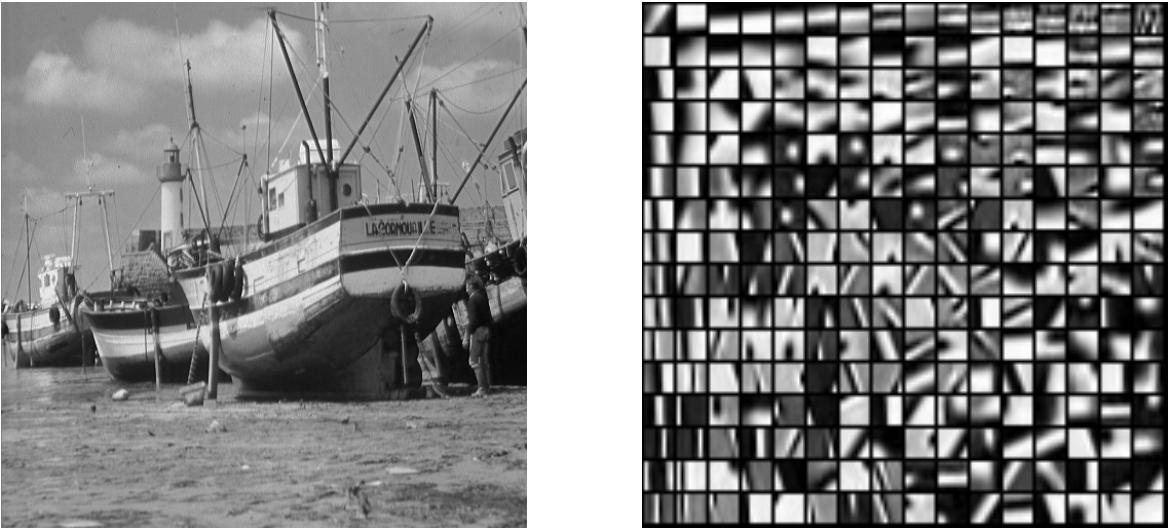
\includegraphics[width=\textwidth]{boats_dico.jpg}%\\            
  \end{center}
  \begin{itemize}
   \item  Dictionary trained on a \alert{noisy} version of the image
  \end{itemize}
From ICCV tutorial\\ {\small \url{http://lear.inrialpes.fr/people/mairal/tutorial_iccv09/tuto_part2.pdf}}
\end{frame}

\begin{frame}
  \frametitle{Applications: denoising}
  \begin{center}
   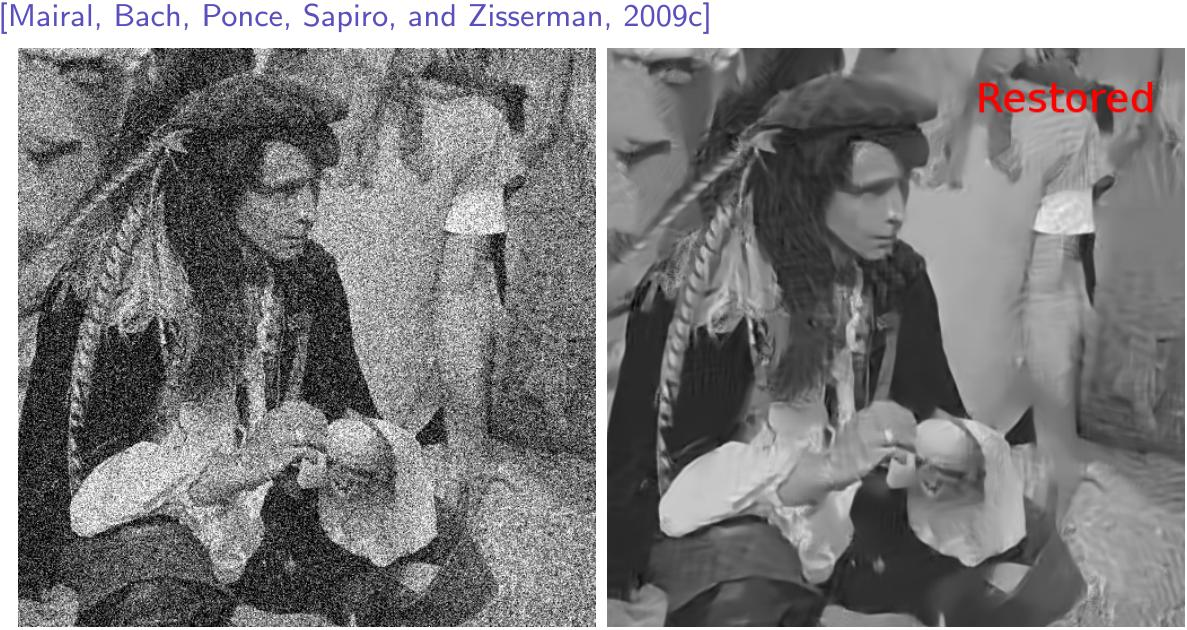
\includegraphics[width=\textwidth]{pirate.jpg}%\\            
  \end{center}
  \begin{itemize}
   \item  Dictionary trained on a \alert{noisy} version of the image
  \end{itemize}
From ICCV tutorial\\ {\small \url{http://lear.inrialpes.fr/people/mairal/tutorial_iccv09/tuto_part2.pdf}}
\end{frame}

\begin{frame}
  \frametitle{Applications: inpainting (1)}
  \begin{center}
   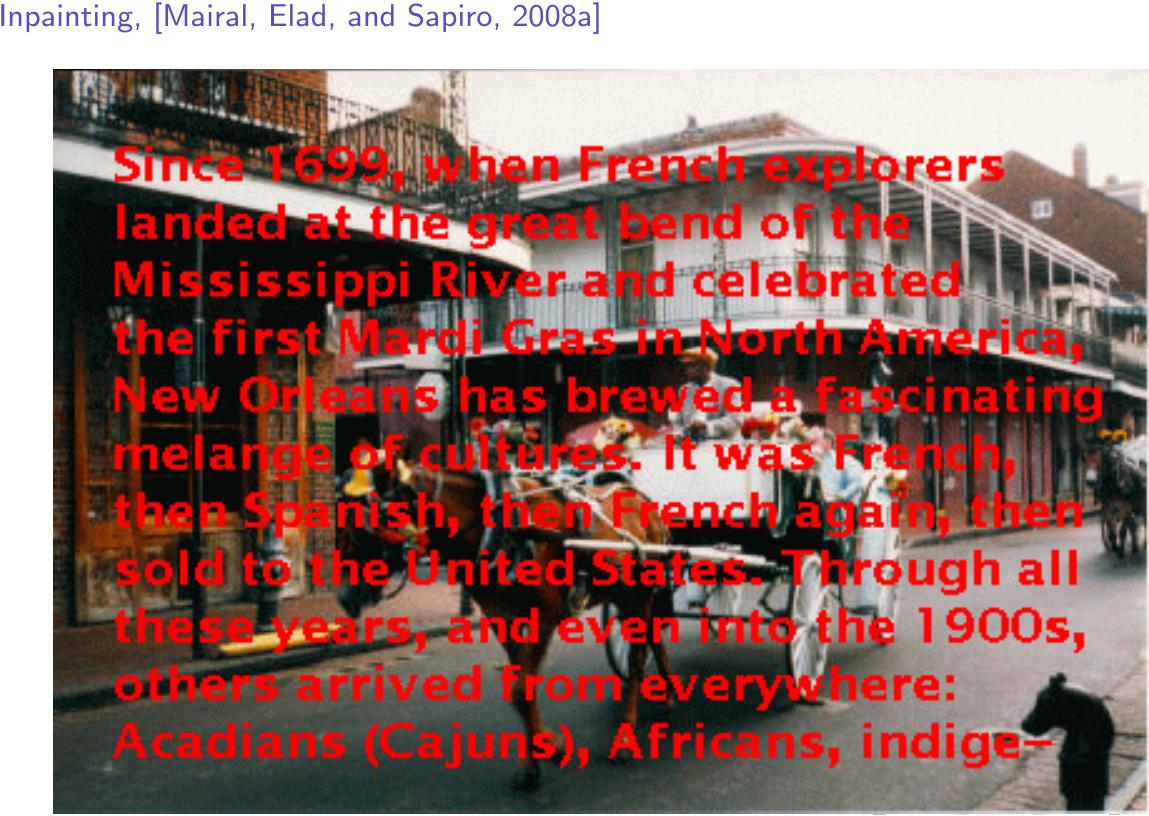
\includegraphics[width=.8\textwidth]{western_text.jpg}%\\            
  \end{center}
  \begin{itemize}
   \item  Dictionary trained on the image with \alert{missing} data
  \end{itemize}
  \scriptsize{
From ICCV tutorial  \url{http://lear.inrialpes.fr/people/mairal/tutorial_iccv09/tuto_part2.pdf}}
\end{frame}

\begin{frame}
  \frametitle{Applications: inpainting (2)}
  \begin{center}
   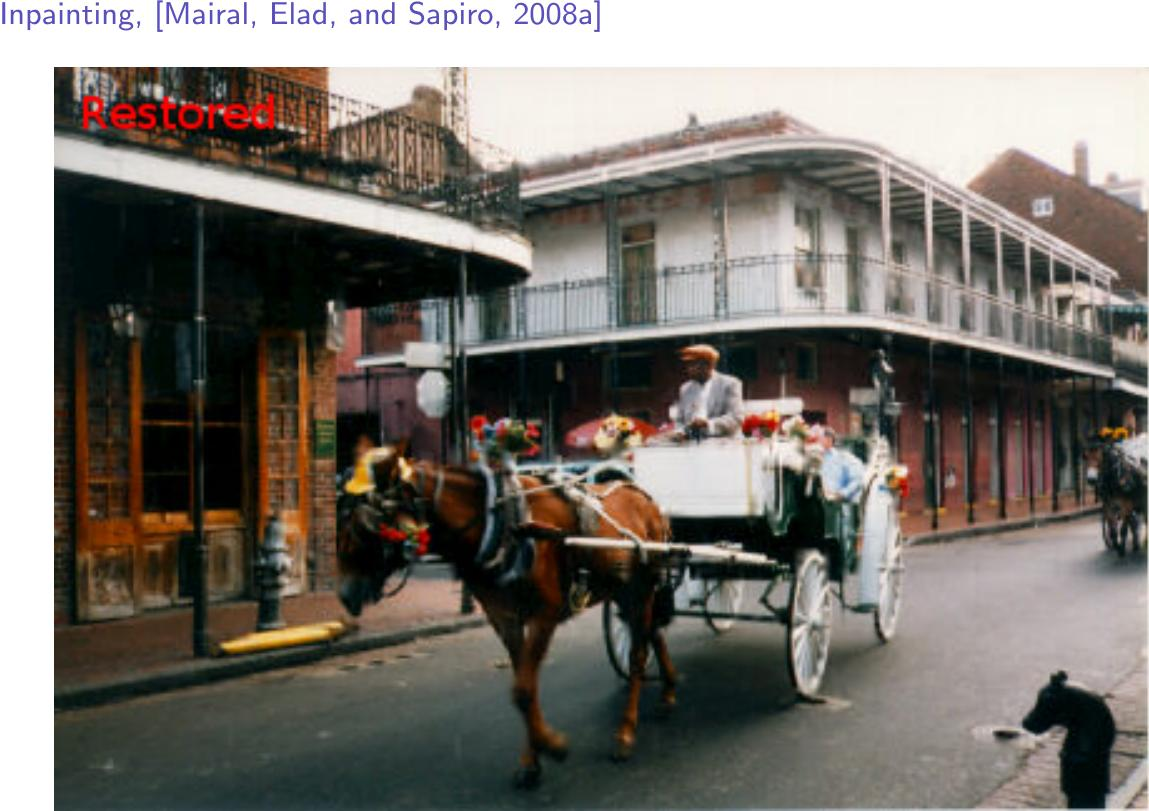
\includegraphics[width=.8\textwidth]{western_restored.jpg}%\\            
  \end{center}
  \begin{itemize}
   \item  Dictionary trained on the image with \alert{missing} data
  \end{itemize}
  \scriptsize{
From ICCV tutorial  \url{http://lear.inrialpes.fr/people/mairal/tutorial_iccv09/tuto_part2.pdf}}
\end{frame}

\end{document}
